\documentclass[a6paper]{article}
\usepackage{polyglossia}
\usepackage[margin=5mm]{geometry}
\usepackage{graphicx}
\setdefaultlanguage{marathi}
\setotherlanguages{english, sanskrit}
%\setmainfont[Mapping=velthuis-sanskrit,Script=Devanagari,Language=Sanskrit]{Shobhika}
\newfontfamily\englishfont{Arial}
\newfontfamily\devanagarifont{Sanskrit Text}
\newfontfamily\marathifont[Mapping=velthuis-sanskrit,Script=Devanagari,Language=Marathi]{Sanskrit Text}
\newfontfamily\sanskritfont[Mapping=velthuis-sanskrit,Script=Devanagari,Language=Sanskrit]{Sanskrit Text}
% make sure ~ as non-breaking space doesn't interfere with velthuis-sanskrit mapping
\edef~{\string~}
\pagenumbering{gobble}
\setlength{\parindent}{0pt}% Remove paragraph indent
\usepackage[skip=\medskipamount]{parskip}
\usepackage{xcolor}
\usepackage{hyperref}
\renewcommand\UrlFont{\ttfamilylatin}
\newcommand \eng[1]{
    \textenglish{#1}
}
% hyphenation https://tex.stackexchange.com/a/177179/64425
\tolerance=1
\emergencystretch=\maxdimen
\hyphenpenalty=10000
\hbadness=10000

\hypersetup{
    colorlinks=true,
    linkcolor=blue,
    filecolor=magenta,
    citecolor=blue,
    urlcolor=purple,
}

\begin{document}

\begin{center}
    {\Large "subhaaste panthaana.h santu!}
\end{center}
\hspace*{\fill} pu.nenagaram 

\hspace*{\fill} ma"ngalavaasara.h 20-12-2022 

v.r.saaliivi"svanaathau a"sviniicetanau ca saadara.m vandaavahe|

devikaasaumitrayo.h vivaahapriityartha.m abhinandanaani| ma"ngalakaale gata"sanivaasare aavaa.m 
vivaahasthaane durbhaagyava"saat anupasthitau iti satyam|
k.samyetaam|
kintu bhaavaruupe.na na tu mi.s.taannamitarejananyaayena tatraiva aasaava tadaa! 
bhavataa pre.sitaa sa.msk.rtasaundarye.na sa.msk.rtamaadhurye.na raghuva.m"saadi"slokena ca sajjitaa 
aavaahanapatrikaa aavayo.h santo.saarthameva! bahu dhanyavaadaa.h|

navapari.niitaabhyaa.m dampatiibhyaa.m haardaa.h "subhaa"sayaa.h| vaivaahikajiivana.m saukhyapuur.na.m bhuuyaat|

bhavadiiyau

nuupuraanitinau|

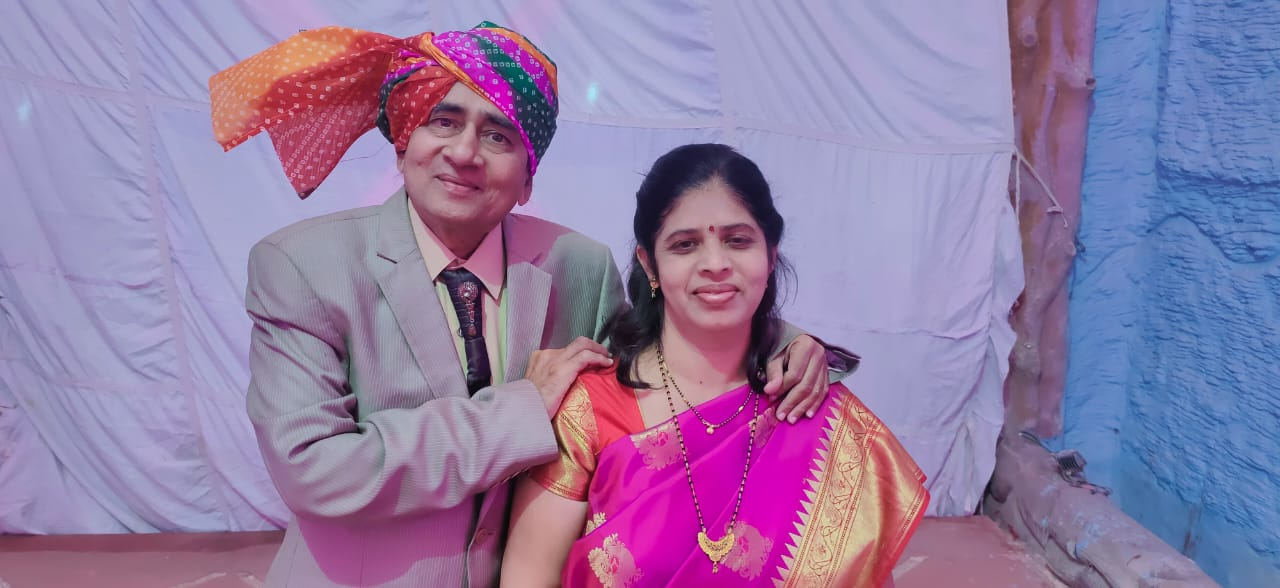
\includegraphics[width=0.5\textwidth]{pariNaya-p2.png}
%TC:ignore



%TC:endignore
\end{document}
